\documentclass[10pt,a4paper]{article}
\usepackage[utf8]{inputenc}

% IDIOMA ESPAÑOL
\usepackage[spanish]{babel}

\usepackage{amsmath}
\usepackage{amsfonts}
\usepackage{amssymb}

%GRAFICOS
\usepackage{graphicx}

% TABLAS
\usepackage{multirow}

% BIBLIOGRAFIA
\usepackage[backend=biber]{biblatex}
\addbibresource{bibliografia.bib}

% HIPERVINCULOS
\usepackage{hyperref}

\usepackage[left=2cm,right=2cm,top=2cm,bottom=2cm]{geometry}
\author{Fernández, Gonzalo Gabriel}
\title{Trabajo Final Inteligencia Artificial I – año 2018: Visión Artifical}

\begin{document}

% TÍTULO
\maketitle

% RESUMEN
\begin{abstract}
El presente trabajo sobre visión artificial fue realizado como trabajo final de la cátedra Inteligencia Artificial I, de la Facultad de Ingeniería de la Universidad Nacional de Cuyo.

Consiste en el diseño e implementación de un agente capaz de clasificar frutas, bananas, naranjas y limones, en base a fotografías. Se realiza un breve estudio teórico del agente. En la implementación se analiza el procesado de imágenes en sus diferentes etapas: filtrado, segmentado y extracción de características. Para clasificar las imágenes se utilizan algoritmos de aprendizaje K-means y K-nn, y se hace un estudio de desempeño comparativo entre los dos algoritmos. El lenguaje de programación utilizado a lo largo del proyecto es Python.

Como objetivo final se desea obtener un agente que en un entorno con condiciones controladas se desempeñe con un rendimiento por encima de las exigencias.
\end{abstract}

% INTRODUCCION
\section{Introducción}

\subsection{Visión Artificial\label{vision}}
``\textit{La \textbf{visión artificial} o visión por ordenador es una disciplina científica que incluye métodos para adquirir, procesar, analizar y comprender las imágenes del mundo real con el fin de producir información numérica o simbólica para que puedan ser tratados por un ordenador.}'' Wikipedia, la Enciclopedia Libre.
``\textit{En la visión por ordenador, intentamos describir el mundo que vemos en una o más imágenes e intentamos reconstruir sus propiedades, tal como la forma, iluminación y distribuciones de color.}'' \textcite{szeliski}

\subsection{Problema a resolver}
Se está desarrollando un \textbf{sistema de reconocimiento de frutas por visión artificial} con la intención de agilizar el proceso de cobro en las cajas de un supermercado. Para ello se
pide desarrollar un agente prototipo que pueda \textbf{reconocer bananas, naranjas y limones} a partir de fotografías.

Las condiciones impuestas son que las \textbf{imágenes deben tomarse en escala de grises}, y que debe utilizarse los \textbf{algoritmos K-means y K-nn} para realizar la clasificación, y a partir de los resultados obtenidos sugerir uno de ellos para ser implementado.

Es recomendado una extracción de características mediante la aplicación de un análisis textural a través de una matriz de covarianza con un vector de características que se construya a partir de los autovalores de dicha matriz.

% ESPECIFICACIÓN DEL AGENTE
\section{Especificación del agente}
La descripción del agente y su entorno se realiza en base a la clasificación de \textcite{rusellnorving}, Capítulo 1.

\subsection{Tipo de agente}
El agente es \textbf{racional}: ``\textit{En cada posible secuencia de percepciones, un agente racional deberá emprender aquella acción que supuestamente maximice su medida de rendimiento, basándose en las evidencias aportadas por la secuencia de percepciones y en el conocimiento que el agente mantiene almacenado.}'' \textcite{rusellnorving}. Es \textbf{no omnisciente}, ya que no conoce el resultado de sus acciones, no posee total información de todo su entorno. El objetivo de utilizar algoritmos como K-means o K-nn es que el agente \textbf{aprenda} a lo largo de sus percepciones, y también que sea \textbf{autónomo}, y pueda apoyarse más en la experiencia adquirida gracias a sus propias percepciones que en el conocimiento inicial proveído por el diseñador.

El agente es un \textbf{agente que aprende}, debido al tipo de algoritmos que utiliza. La base de datos provee un "modelo" del mundo, y los algoritmo también actúan en base a una "utilidad" que se analiza más adelante.

\subsection{Tabla REAS: Rendimiento, Entorno, Actuadores, Sensores}
\begin{itemize}
\item \textbf{Tipo de Agente:}

Computadora, microcontrolador o microprocesador en el cuál se encuentran los algoritmos entrenados, y los dispositivos de \textit{entrada y salida}, o más correcto en éste análisis, \textit{sensores y actuadores}: cámara fotográfica, monitor, etc.

\item \textbf{Medidas de Rendimiento:}

A la hora de implementar los algoritmos, se posee una base de datos con toda la información recopilada etiquetada por clase, en este caso fotografías de bananas, naranjas y limones. A esta base de datos se la divide en dos conjuntos: entrenamiento y testeo. El conjunto de testeo nos permitirá dar una medida de rendimiento del agente, siendo esta medida la cantidad de predicciones correctas de todos los elementos de testeo.

\item \textbf{Entorno:}

El entorno del agente será el área donde esté ubicada la fruta a la hora de tomar la fotografía, y la fruta en sí. Al entorno también lo integran todos los factores externos que se exponen más adelante, como luminosidad, fondo, calidad de la fruta, etc.

\item \textbf{Actuadores:}

El actuador del agente es sencillamente el medio por el que éste se comunicará con el usuario para darle a conocer su predicción. Puede ser un display, una consola, una señal luminosa o auditiva, o cualquier otro medio que resulte adecuado.

\item \textbf{Sensores:}

El sensor del agente es la cámara fotográfica que tomará la imagen de la fruta. Esto es así, si se considera la cámara fotográfica como parte del agente. Sin embargo, la imagen puede provenir de otras fuentes externas que no se consideren parte del agente. En este caso, podría considerarse como sensor las herramientas (librerías y sus funciones) que nos permiten procesar la imagen en el formato que se reciba (\textit{PNG, JPEG}), en un formato de información con la que el agente puede operar.

\end{itemize}
 
\subsection{Propiedades del entorno de trabajo}
\begin{itemize}
\item \textbf{Parcialmente observable:}

El entorno es parcialmente observable, ya que el agente está recibiendo una representación del mundo real, en dos dimensiones; una imagen que describe el entorno mediante un arreglo discreto de pixeles con un determinado valor. Esta limitación está asociada a lo explicado en la introducción, sección \ref{vision}.

\item \textbf{Estocástico:}

Que el entorno sea parcialmente observable hace que desde el punto de vista del agente, el entorno parezca en gran medida estocástico. Debido a la gran diferencia entre la representación del entorno en la imagen y el mundo real, el agente nunca puede estar seguro de los hechos en el exterior.  

\item \textbf{Episódico:}

El entorno es episódico ya que el estado del entorno en un determinado instante de tiempo no depende de la secuencia de estados previos. La cámara fotográfica tomará imágenes de las frutas en el orden que se le presenten, y este orden no tiene ninguna inferencia en el desempeño del agente.

\item \textbf{Estático:}

El entorno no cambia mientras el agente está deliberando. Una vez tomada la fotografía, comenzado el procesamiento el agente se aísla en cierto modo del entorno.

\item \textbf{Discreto:}

Que el entorno sea discreto está relacionado con que también es estático. El agente no interactúa en tiempo real con el entorno, sino solo en el corto lapso en que toma la fotografía.

\item \textbf{Agente individual:}

El entorno es agente individual ya que en todo el proceso de interacción agente-entorno, el único ente racional es el agente.

\end{itemize}

% PLANIFICACIÓN
\section{Planificación del proyecto}
Se realizó un análisis de las tareas a realizar para aumentar la productividad del trabajo. Aprovechando la oportunidad, se aplicaron conceptos de planificación aprendidos en la cátedra.

En la figura \ref{plan-parcial}, se expone el \textbf{plan de orden parcial} realizado, con las tareas principales a resolver, tanto para el informe como el código en sí.

\begin{figure}[h]
\centering
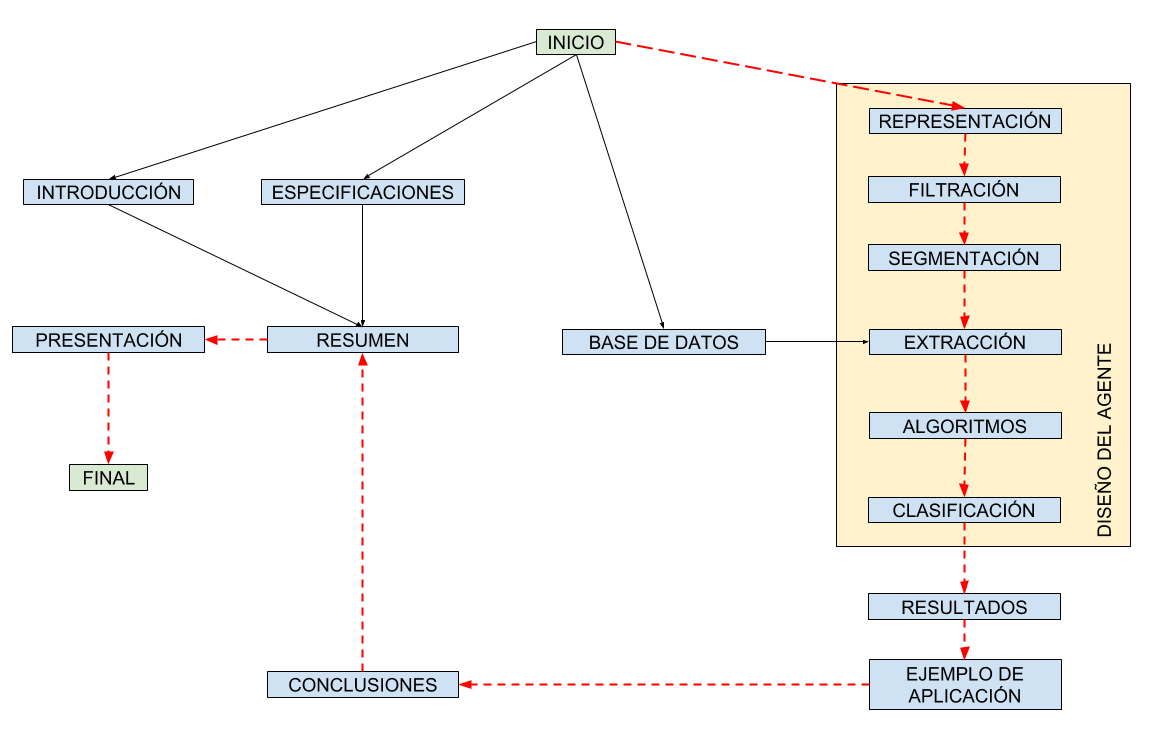
\includegraphics[width=0.8\textwidth]{imgs/plan-parcial.png}
\caption{Plan de orden parcial para la realización del proyecto. Las flechas rojas de trazos indican el camino crítico encontrado.}
\label{plan-parcial}
\end{figure}

Si se observa la figura \ref{plan-parcial}, las flechas rojas de trazos indican el \textbf{camino crítico}, en el cuál se encuentran las tareas sin tiempo de relajación, por lo que deben realizarse sin demoras. Éste camino crítico está dado básicamente por la implementación del código.

\section{Diseño del agente}
Se inicia el proyecto eligiendo con qué lenguaje de programación se encarará. Se decide utilizar \textbf{\textit{Python}}, por ser tan popular en las disciplinas relacionadas con inteligencia artificial. Entre las opciones, además de \textit{Python} se consideró utilizar \textit{Matlab} o \textit{R}.

Siendo la primer experiencia con análisis de imágenes, la primer interrogante que surge es cómo obtener de una imagen cruda de la fruta, un vector representativo de todas sus características que sea de utilidad como entrada a los algoritmos K-means y K-nn.

En base a distintas referencias, se decide dividir el problema con cuatro etapas principales: \textbf{representación de la imagen} en un arreglo de números fáciles de computar, \textbf{filtrar} la imagen para eliminar ruido, \textbf{segmentar} la imagen para resaltar características que puede ser relevantes para el posterior análisis y la \textbf{extracción de características}, donde como resultado se obtendría un vector representativo de la imagen capaz de ser una de las tantas entradas a los algoritmos antes mencionados, \textcite{SciPy2018}.

Las librerías que se utilizaron para resolver el problema propuesto son \textit{SciPy} y \textit{OpenCV}.

\href{https://www.scipy.org/}{SciPy} es un ecosistema basado en \textit{Python} de software \textit{open-source} para matemática, ciencia e ingeniería. Los paquetes que se utilizaron específicamente en este trabajo son:

\begin{itemize}
\item \href{http://www.numpy.org/}{NumPy}: Es un paquete para computación científica. Contiene herramientas como arreglos n-dimensionales, funciones sofisticadas, herramientas para integrar \textit{C/C++} y \textit{Fortran}, álgebra linear, transformada de Fourier, operaciones random, etc.

\item \href{https://matplotlib.org/}{Matplotlib}: Es una librería para gráficos 2D con calidad de publicación.

\item \href{https://ipython.org/}{IPython}: Provee una arquitectura para computación interactiva con una potente consola, un kernel para \textit{Jupyter}, visualización de datos interactiva, etc.
\end{itemize}

\href{https://opencv.org/}{OpenCV} (Open Source Computer Vision Library), es una librería de funciones para \textit{C++}, \textit{Python} y otros lenguajes, donde su propósito principal es la visión artificial en tiempo real.

Para exponer el código y la investigación realizada de una forma clara, sensilla y reproducible, se utilizó \href{https://jupyter.org/}{Jupyter}. Jupyter es una aplicación web open-source que permite crear y compartir documentos con bloques de código embebido, ecuaciones, gráficos y texto descriptivo.

La descripción más específica y técnica de la implementación se encuentra en los diferentes \textit{Jupyter notebook} del proyecto. Para acceder a ellos, ir al link provisto correspondiente.

\subsection{Representación adecuada de la información}
\textit{Jupyter notebook}: \href{./01-representacion.ipynb}{01-representacion}. En el caso de no disponer del proyecto completo: \href{https://github.com/FernandezGFG/fruit-classifier/blob/master/01-representacion.ipynb}{link de GitHub}.

Al analizar la conversión a escala de grises se utiliza la fórmula:
\begin{equation}
Y'_{709}=0.2125R'+0.7154G'+0.0721B'
\label{gris}
\end{equation}

La ecuación \ref{gris} se obtiene de \textcite{szeliski}, capitulo 2 ``Image Formation'', 2.3 ``The digial camera''.

El resultado obtenido en esta etapa es la imagen en escala de grises en un tamaño normalizado, a partir de la fotografía original recibida por el agente. Se puede observar un ejemplo en la figura \ref{resultado-01}. El proceso se puede hacer por medio de la librería \textit{skimage} o también con la librería \textit{OpenCV} (más específicamente \textit{cv2}).

\begin{figure}[h]
\centering
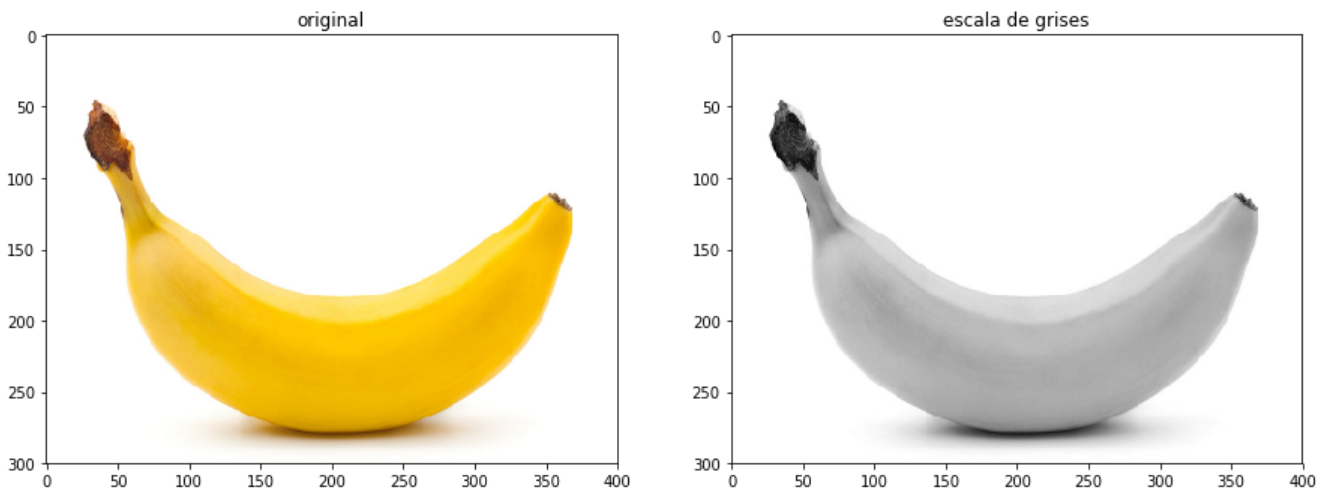
\includegraphics[width=0.7\textwidth]{imgs/resultado-01.png}
\caption{Resultado obtenido en \textit{Jupyter notebook} \href{./01-representacion}{01-representacion}.}
\label{resultado-01}
\end{figure}

\subsection{Filtrado de imágenes}
\textit{Jupyter notebook}: \href{./02-filtracion.ipynb}{02-filtracion}. En el caso de no disponer del proyecto completo: \href{https://github.com/FernandezGFG/fruit-classifier/blob/master/02-filtracion.ipynb}{link de GitHub}.

De \textit{Wikipedia, la Enciclopedia Libre}: ``Es el conjunto de técnicas englobadas dentro del preprocesamiento de imágenes cuyo objetivo fundamental es obtener, a partir de una imagen origen, otra final cuyo resultado sea más adecuado para una aplicación específica mejorando ciertas características de la misma que posibilite efectuar operaciones del procesado sobre ella. Los principales objetivos que se persiguen con la aplicación de filtros son:
\begin{itemize}
\item Suavizar la imagen: reducir la cantidad de variaciones de intensidad entre píxeles vecinos.
\item Eliminar ruido: eliminar aquellos píxeles cuyo nivel de intensidad es muy diferente al de sus vecinos y cuyo origen puede estar tanto en el proceso de adquisición de la imagen como en el de transmisión.
\item Realzar bordes: destacar los bordes que se localizan en una imagen.
\item Detectar bordes: detectar los pixeles donde se produce un cambio brusco en la función intensidad.
\end{itemize}

Por tanto, se consideran los filtros como operaciones que se aplican a los pixeles de una imagen digital para optimizarla, enfatizar cierta información o conseguir un efecto especial en ella.''.

En este trabajo se estudiaron los siguientes filtros:
\begin{itemize}
\item \textit{Gaussian}: Altamente recomendado y utilizado ampliamente para eliminar ruido, reducir detalle de las fotografías, y como una etapa de preprocesamiento de imágenes.
\item \textit{Diferencial}: Se utiliza para obtener los cambios en la intensidad de la imagen. El resultado es el gradiente, en la dirección que se realizó el filtro, de la intensidad de la imagen. Es un primer paso al detectar bordes de la imagen.
\item \textit{Sobel}: Es un filtro muy utilizado para la detección de bordes. Es una aproximación al gradiente de la imagen. En el trabajo se realiza una comparación entre el filtro \textit{Sobel} y la composición de dos filtros \textit{diferenciales} ortogonales, obteniendo resultados similares. En la librería \textit{OpenCV} a esta composición se le denomina filtro \textit{Laplacian}, por estar relacionado con la ecuación de Laplace.
\item \textit{Median}: Este filtro a diferencia de los anteriores es no lineal. Se utiliza de una forma similar al filtro \textit{Gaussian}, para reducir ruido en las imágenes.
\end{itemize}

Los resultados obtenidos en esta etapa es la imagen en escala de grises (o no) en un tamaño normalizado, filtrada por \textit{Gaussian} y/o \textit{Sobel} dependiendo la necesidad, a partir de la fotografía original recibida por el agente. Se puede observar un ejemplo en la figura \ref{resultado-02}. El proceso se puede hacer por medio de la librería \textit{skimage} o también con la librería \textit{OpenCV} (más específicamente \textit{cv2}).

\begin{figure}[h]
\centering
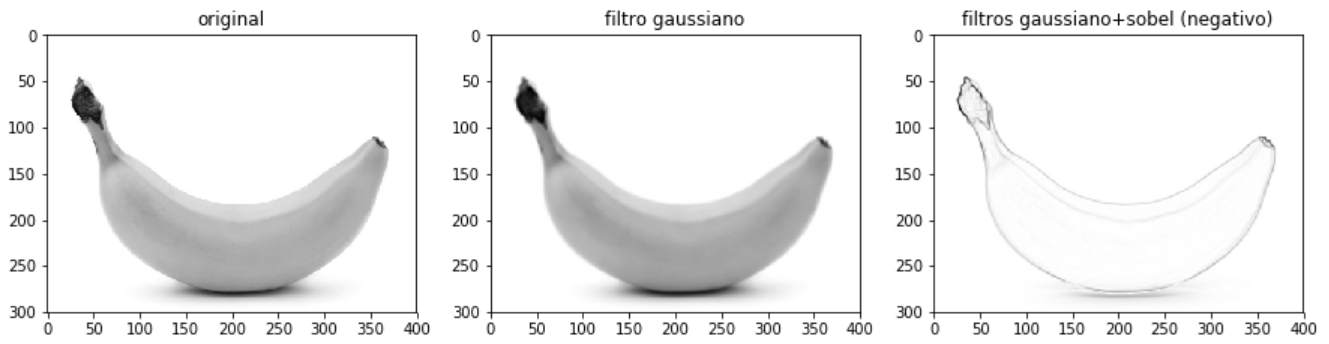
\includegraphics[width=\textwidth]{imgs/resultado-02.png}
\caption{Resultado obtenido en \textit{Jupyter notebook} \href{./02-filtracion}{02-filtracion}.}
\label{resultado-02}
\end{figure}

\subsection{Segmentado de imágenes}
\textit{Jupyter notebook}: \href{./03-segmentacion.ipynb}{03-segmentacion}. En el caso de no disponer del proyecto completo: \href{https://github.com/FernandezGFG/fruit-classifier/blob/master/03-segmentacion.ipynb}{link de GitHub}.

El resultado del proceso de segmentación, es una imagen binaria que contendría los bordes del objeto a analizar. Esto puede utilizarse o no, según el método de extracción de características que se utilice. Se puede observar un ejemplo en la figura \ref{resultado-03}. El proceso se puede hacer por medio de la librería \textit{skimage} o también con la librería \textit{OpenCV} (más específicamente \textit{cv2}).

\begin{figure}[h]
\centering
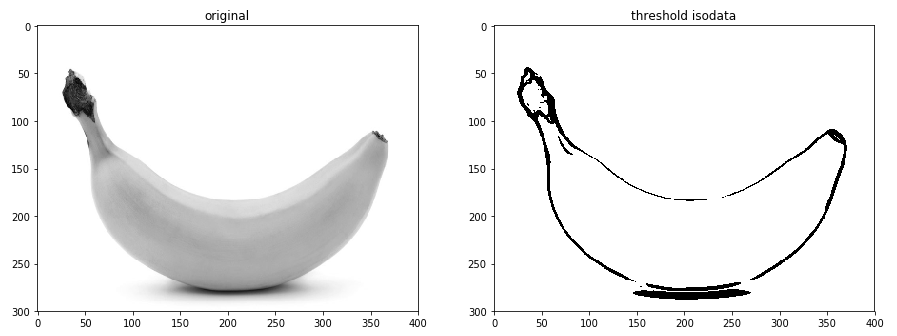
\includegraphics[width=0.7\textwidth]{imgs/resultado-03.png}
\caption{Resultado obtenido en \textit{Jupyter notebook} \href{./03-segmentacion}{03-segmentacion}.}
\label{resultado-03}
\end{figure}

\subsection{Base de datos}
A la hora de obtener resultados se utilizó dos bases de datos: La primera es una base de datos proveída por Kaggle: \href{https://www.kaggle.com/moltean/fruits}{Fruit 360 Kaggle dataset}. \href{https://www.kaggle.com}{Kaggle} es una comunidad online de \textit{Data Science} y \textit{Machine Learning} de \textit{Google, Inc.}. Permite a los usuarios encontrar y publicar \textit{data sets}, trabajar con otras personas expertas en el tema e inclusive participar en competencias y desafíos relacionados con el análisis de datos. El problema de éste \textit{data set}, es que las frutas están diseñadas con herramientas de software, es decir, no son fotografías de frutas reales. Ésto hace que la diferencia con una fotografía tomada por el usuario sea muy grande. Sin embargo, fue de mucha utilidad para una primera observación de resultados y confirmar que las decisiones tomadas hasta el momento son acertadas. Luego de trabajar con este \textit{data set} de Kaggle, se construyo uno propio a partir de fotografías de frutas reales comprobando esta gran diferencia de resultados. En el cuadro \ref{dataset}, puede observarse la cantidad de imágenes utilizada.

\begin{table}[h]
\centering
\begin{tabular}{|c|c|c|c|c|c|c|c|}
\hline
\multirow{2}{*}{\textbf{}} & \multicolumn{3}{c|}{\textbf{Train}} & \multicolumn{3}{c|}{\textbf{Test}} &  \\ \cline{2-8} 
 & \textbf{Banana} & \textbf{Naranja} & \textbf{Limón} & \textbf{Banana} & \textbf{Naranja} & \textbf{Limón} & \textbf{Total} \\ \hline
\textbf{Kaggle} & 490 & 479 & 492 & 166 & 160 & 164 & 1951 \\ \hline
\textbf{Personal} & 132 & 138 & 130 & 131 & 138 & 130 & 799 \\ \hline
\end{tabular}
\caption{Cantidad de imágenes en los diferentes \textit{data sets}.}
\label{dataset}
\end{table}

Para las imágenes de la base de datos propia, se tomo las fotografías de las diferentes frutas individuales, sobre una hoja de papel blanca, con \textit{flash} y buena iluminación del ambiente.

\subsection{Extracción de características}
\textit{Jupyter notebook}: \href{./04-extraccion.ipynb}{04-extraccion}. En el caso de no disponer del proyecto completo: \href{https://github.com/FernandezGFG/fruit-classifier/blob/master/04-extraccion.ipynb}{link de GitHub}.

Para la extracción de características se utilizaron diferentes métodos:
\begin{itemize}
\item \textbf{Histogram of oriented gradients (HOG):} Es utilizado en visión por computador y procesado de imágenes con el propósito de detección de objetos. Resultados obtenidos (reducidos a media y desviación estándar) en la figura \ref{hog}.

\begin{figure}[h]
\centering
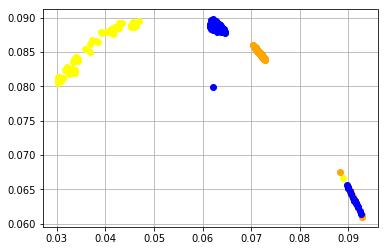
\includegraphics[width=0.55\textwidth]{imgs/resultado-04_hog.png}
\caption{Histogram of Oriented Gradients (HOG) para la base de datos, reducida a media y desviación estándar.}
\label{hog}
\end{figure}

\item \textbf{Hu Moments:} Generalmente es utilizado para la extracción de la silueta o contorno del objeto en la imagen. Da una valorización de la forma de éste, que puede ser medida comparando vectores de características \textit{Hu Moments} a través de distancias, por ejemplo. Resultados obtenidos (reducidos a media y desviación estándar) en la figura \ref{hu_moments}.

\begin{figure}[h]
\centering
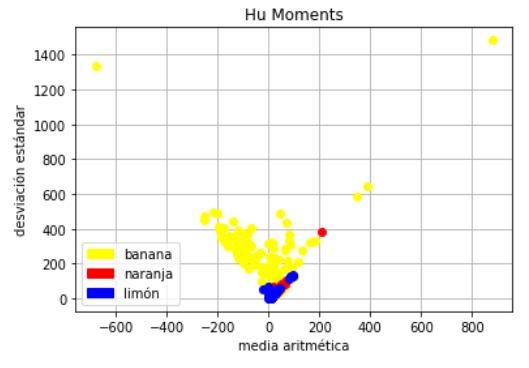
\includegraphics[width=0.55\textwidth]{imgs/resultado-04_hm.png}
\caption{Hu Moments para la base de datos, reducida a media y desviación estándar.}
\label{hu_moments}
\end{figure}

\item \textbf{Haralick Textures:} Las características de textura están basadas en estadísticas  que resumen la distribución de frecuencia relativa (que describe cuán a menudo un tono gris aparece en una zona espacial específica en relación a otro tono de gris en la imagen), \textcite{haralick}. Resultados obtenidos (reducidos a media y desviación estándar) en la figura \ref{haralick_textures}.

\begin{figure}[h]
\centering
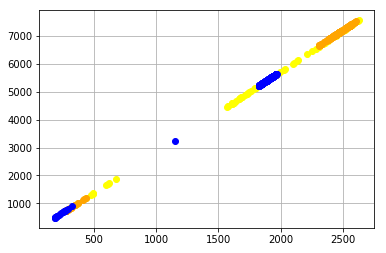
\includegraphics[width=0.55\textwidth]{imgs/resultado-04_ht.png}
\caption{Haralick Textures para la base de datos, reducida a media y desviación estándar.}
\label{haralick_textures}
\end{figure}

\item \textbf{Color Histogram:} Es sencillamente una representación de la distribución de colores en la imágen. En imágenes digitales, el histograma de color representa el número de pixeles que tienen determinado color en una lista fija con el rango de colores. Resultados obtenidos (reducidos a media y desviación estándar) en la figura \ref{color_histogram}.

\begin{figure}[h]
\centering
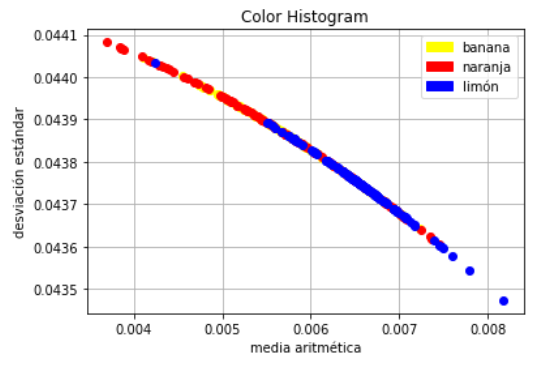
\includegraphics[width=0.55\textwidth]{imgs/resultado-04_ch.png}
\caption{Color Histogram para la base de datos, reducida a media y desviación estándar.}
\label{color_histogram}
\end{figure}

\end{itemize}

\subsection{Implementación de los algoritmos de clasificación}
\textit{Jupyter notebook}: \href{./05-algoritmos.ipynb}{05-algoritmos}. En el caso de no disponer del proyecto completo: \href{https://github.com/FernandezGFG/fruit-classifier/blob/master/05-algoritmos.ipynb}{link de GitHub}.

En esta etapa se implementan los dos algoritmos de clasificación a utilizar: \textbf{K-nn (K-nearest neighbors)} y \textbf{K-means}. Su descripción técnica se encuentra detalladamente en el \textit{jupyter notebook} correspondiente.

\subsection{Clasificación de la información}
\textit{Jupyter notebook}: \href{./06-clasificacion.ipynb}{06-clasificacion}. En el caso de no disponer del proyecto completo: \href{https://github.com/FernandezGFG/fruit-classifier/blob/master/06-clasificacion.ipynb}{link de GitHub}.

En este último paso, a diferencia de la implementación inicial, no se trabaja con una imagen ejemplo, sino con toda la base de datos. Se divide toda la información en dos subconjuntos, uno para el entrenamiento de los algoritmos y otro de testeo para calificar su desempeño.

Se ejecuto numeradas veces con el objetivo de comparar resultados utilizando filtros, segmentación y diferentes métodos de extracción de características. Los resultados obtenidos se exponen en la sección \ref{resultados}.

% CÓDIGO
\section{Código}
El código de todo lo previamente explicado se encuentra expuesto junto al análisis teórico, en los diferentes \textit{Jupyter notebook}.

El código final obtenido posterior a la etapa de diseño se encuentra en la carpeta \href{./src/}{src} del proyecto. Consiste en un conjunto de programas \textit{python} que ejecutan las diferentes etapas. Sin embargo, para simplicidad de ejecución, se escribió dos \textit{scripts} en \textit{bash} nombrados \href{./run-test}{run-test} y \href{./run-project}{run-project}, que ejecutan los programas en \textit{python} en la secuencia correcta junto con otras acciones necesarias para una ejecución limpia.

\begin{itemize}
\item \textbf{run-test:} Ejecutar el \textit{script} para entrenar la base de datos y proceder con el testeo del proyecto. Una barra de progreso provee de forma gráfica los resultados finales obtenidos. Se ejecutan ambos algoritmos \textit{K-means} y \textit{K-nn}. El comando es, desde la carpeta principal del proyecto donde se encuentra \textit{run-test}, como el que sigue:
\begin{verbatim}
./run-test
\end{verbatim}
\item \textbf{run-project:} Ejecutar el \textit{script} para clasificar una determinada imagen, la ruta donde se encuentra esta imagen es un parámetro del programa. El comando es, desde la carpeta principal del proyecto donde se encuentra \textit{run-project}, como el que sigue:
\begin{verbatim}
./run-project <ruta de la imagen a clasificar>
\end{verbatim}
\end{itemize}

En la figura se expone la estructura de carpetas del proyecto.

\begin{figure}[h]
\centering
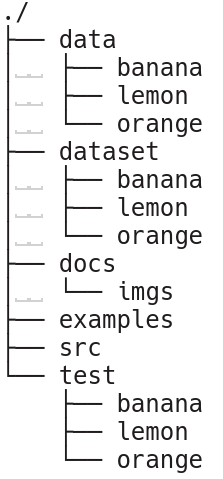
\includegraphics[scale=0.4]{imgs/folders-structure.png}
\caption{Estructura de carpetas del proyecto.}
\label{folders}
\end{figure}

Las \textbf{dependencias}, es decir, las librerías necesarias de \textit{Python} para poder ejecutar el proyecto son: \textit{Numpy}, \textit{Skimage}, \textit{cv2} (OpenCV), \textit{Mahotas}, \textit{Pickle}, \textit{sys} y \textit{random}.

% RESULTADOS
\section{Resultados\label{resultados}}
Los resultados obtenidos son en referencia a la base de datos utilizada. Como se mencionó previamente, se divide en dos subconjuntos de imágenes: uno de entrenamiento y otro de testeo. Los resultados se dan en \textbf{porcentaje de aciertos en predicciones del conjunto de testeo}.

El objetivo del conjunto de testeo es dar una noción de que métodos de extracción de características, filtros y segmentados, dan mejores resultados y tomar una decisión en el diseño final del agente en base a ello. 

En el cuadro \ref{resultado-knn} se exponen los resultados obtenidos con los diferentes \textit{data sets} para el algoritmo \textit{K-nn}.

\begin{table}[h]
\centering
\begin{tabular}{|c|c|c|c|c|c|}
\hline
\multicolumn{2}{|c|}{\textbf{Análisis de imagen}} & \multicolumn{2}{c|}{\textbf{Kaggle}} & \multicolumn{2}{c|}{\textbf{Personal}} \\ \hline
\textbf{\begin{tabular}[c]{@{}c@{}}Método de extracción\\ de características\end{tabular}} & \textbf{Filtro} & \multicolumn{1}{c|}{\textbf{$K=1$}} & \multicolumn{1}{c|}{\textbf{$K=10$}} & \multicolumn{1}{c|}{\textbf{$K=1$}} & \multicolumn{1}{c|}{\textbf{$K=10$}} \\ \hline
\multirow{2}{*}{\textbf{Haralick Textures}} & Gaussian & \textbf{83.5\%} & 65.7\% & 62.2\% & 49.1\% \\ \cline{2-2}
 & Ninguno & 74.9\% & 63.3\% & \textbf{62.7\%} & 52.4\% \\ \cline{1-2}
\multirow{4}{*}{\textbf{Hu Moments}} & Gaussian + Sobel & 63.3\% & 65.9\% & \textbf{76.9\%} & \textbf{76.7\%} \\ \cline{2-2}
 & Sobel & 93.5\% & 93.5\% & 59.9\% & 71.7\% \\ \cline{2-2}
 & Gaussian & 94.7\% & \textbf{100.0\%} & 68.4\% & \textbf{72.4\%} \\ \cline{2-2}
 & Ninguno & 94.5\% & \textbf{100.0\%} & 67.9\% & \textbf{72.4\%} \\ \cline{1-2}
\multirow{2}{*}{\textbf{Color Histogram}} & Gaussian & 72.4\% & 72.0\% & 47.4\% & \textbf{53.9\%} \\ \cline{2-2}
 & Ninguno & 72.4\% & \textbf{77.3\%} & 46.4\% & 51.4\% \\ \cline{1-2}
\multirow{2}{*}{\textbf{\begin{tabular}[c]{@{}c@{}}Histogram of Oriented\\ Gradients\end{tabular}}} & Gaussian & 94.3\% & 95.9\% & 48.4\% & 56.6\% \\ \cline{2-2}
 & Ninguno & 95.5\% & \textbf{96.9\%} & 37.1\% & 42.1\% \\ \hline
\end{tabular}
\caption{Resultados obtenidos para algoritmo \textit{K-nn}, para diferentes \textit{data sets}; utilizando diferentes métodos de extracción de características y filtros. En porcentaje, la cantidad de predicciones acertadas sobre el total de imágenes en el conjunto de test.}
\label{resultado-knn}
\end{table}

De los resultados puede observarse como aplicar un filtro en el \textit{data set} brindado por Kaggle disminuye la efectividad. Se concluye que es debido a que las imágenes son diseñadas por software, no hay ruido y el filtro lo único que logra es hacer la imagen más borrosa. También puede observarse lo mucho que disminuyen los aciertos al mudarse de un \textit{data set} como el de Kaggle a uno con fotografías propias. Aún así, la diferencia relativa entre métodos de extracción de características y filtros, se mantiene aproximadamente constante. Esto permite poder elegir una combinación entre todas las opciones y estimar que el resultado se puede extrapolar si hay un crecimiento en la cantidad de imágenes en el \textit{data set}, por ejemplo. Otra observación, es que es conveniente utilizar $K=10$ por sobre $K=1$ cuando el \textit{data set} es el de fotografías propias. 

Para el algoritmo \textit{K-means} se obtuvo los resultados del cuadro \ref{resultado-kmeans}.

\begin{table}[h]
\centering
\begin{tabular}{|c|c|c|}
\hline
\textbf{\begin{tabular}[c]{@{}c@{}}Método de extracción\\ de características\end{tabular}} & \textbf{Filtro} & \multicolumn{1}{c|}{\textbf{\begin{tabular}[c]{@{}c@{}}Aciertos / \\ Distribución final\end{tabular}}} \\ \hline
\multirow{2}{*}{\textbf{Haralick Textures}} & Gaussian & \begin{tabular}[c]{@{}c@{}}48.6\%\\ (209, 138, 53)\end{tabular} \\ \cline{2-3}
 & Ninguno & \begin{tabular}[c]{@{}c@{}}43.4\%\\ (36, 144, 220)\end{tabular} \\ \hline
\multirow{4}{*}{\textbf{Hu Moments}} & Gaussian + Sobel & \begin{tabular}[c]{@{}c@{}}41.9\%\\ (4, 353, 43)\end{tabular} \\ \cline{2-3}
 & Sobel & \begin{tabular}[c]{@{}c@{}}40.1\%\\ (4, 45, 351)\end{tabular} \\ \cline{2-3}
 & Gaussian & \begin{tabular}[c]{@{}c@{}}69.4\%\\ (157, 112, 131)\end{tabular} \\ \cline{2-3}
 & Ninguno & \begin{tabular}[c]{@{}c@{}}63.2\%\\ (157, 131, 112)\end{tabular} \\ \hline
\multirow{2}{*}{\textbf{Color Histogram}} & Gaussian & \begin{tabular}[c]{@{}c@{}}49.6\%\\ (60, 142, 198)\end{tabular} \\ \cline{2-3}
 & Ninguno & \begin{tabular}[c]{@{}c@{}}52.4\%\\ (67, 133, 200)\end{tabular} \\ \hline
\multirow{2}{*}{\textbf{\begin{tabular}[c]{@{}c@{}}Histogram of Oriented\\ Gradients\end{tabular}}} & Gaussian & \begin{tabular}[c]{@{}c@{}}59.4\%\\ (129, 128, 143)\end{tabular} \\ \cline{2-3}
 & Ninguno & \begin{tabular}[c]{@{}c@{}}26.8\%\\ (139, 137, 124)\end{tabular} \\ \hline
\end{tabular}
\caption{Resultados obtenidos para el algoritmo \textit{K-means} sobre el \textit{data set} con fotografías propias, utilizando diferentes métodos de extracción de características y filtros. En porcentaje, la cantidad de predicciones acertadas sobre el total de imágenes en el conjunto de test. Debajo del porcentaje, la cantidad de imágenes en cada clase al finalizar el algoritmo.}
\label{resultado-kmeans}
\end{table}

Puede observarse como la cantidad de aciertos para este algoritmo es menor que para el algoritmo \textit{K-nn}. Hay que contemplar que el algoritmo \textit{K-means} es estocástico debido a sus condiciones iniciales aleatorias (por más que se le de una información inicial de cuales son los subconjuntos de cada clase), esto hace que en cada ejecución se obtengan resultados diferentes.

Uno de los motivos por los que el algoritmo \textit{K-means} no tiene tan buen rendimiento, y que también afecta al algoritmo \textit{K-nn}, es que las diferentes clases no forman conjuntos de puntos con límites definidos. Esto puede observarse en las figuras \ref{hog}, \ref{hu_moments}, \ref{haralick_textures} y \ref{color_histogram}. Los subconjuntos de puntos se superponen, entonces al ejecutarse el algoritmo, por cómo esta diseñado, una de las clases tiene predominancia sobre otra (esto puede observarse bien en las distribuciones finales obtenidas en el cuadro \ref{resultado-kmeans}). Esta superposición de conjuntos lógicamente afecta al algoritmo \textit{K-nn} al encerrar los vecinos más cercanos en una circunferencia.

Luego de elegir el algoritmo \textit{K-nn} como el algoritmo con el que se obtienen mejores resultados, y el método \textit{Hu Moments} para extracción de características; se comparó el vector de características crudo, de 7 componentes, con el vector de dos componentes que son la media aritmética y la desviación estándar. El vector de características de 7 componentes da por resultado un \textbf{85.0$\%$} de predicciones correctas en el \textit{data set} de fotografías propias, frente al 76.7$\%$ de predicciones correctas con el vector de 2 componentes. Luego de comprobar esto, con el objetivo de obtener conjuntos con límites aún más marcados, se compararon combinaciones de componentes del vector \textit{Hu Moments}, obteniendo resultados de $91.2\%$ con componentes 0 y 1; y $95.0\%$ con \textbf{tres componentes 0, 1 y 3} como se observa en la figura \ref{final-feature}.

\begin{figure}[h]
\centering
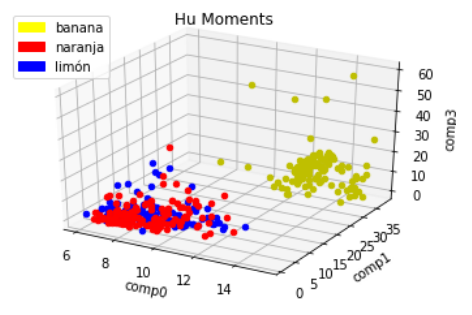
\includegraphics[width=0.6\textwidth]{imgs/final-feature.png}
\caption{Vector de características formado por componentes 0, 1 y 3 del vector \textit{Hu Moments}.}
\label{final-feature}
\end{figure}

Para la elección del $K$ del algoritmo, se ejecuto repetidas veces variando este parámetro desde 1 a 25, obteniendo los valores de la figura \ref{funcion-k}.

\begin{figure}[h]
\centering
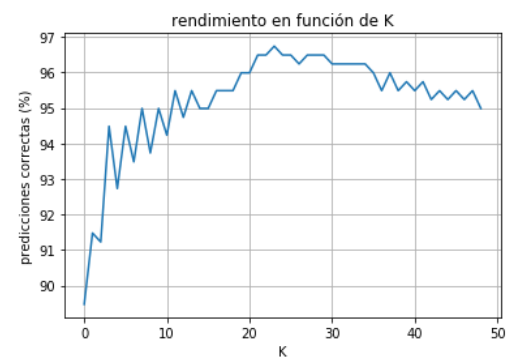
\includegraphics[width=0.6\textwidth]{imgs/funcion-k.png}
\caption{Porcentaje de predicciones correctas en función de $K$ para el algoritmo \textit{K-nn}.}
\label{funcion-k}
\end{figure}

Como puede observarse, los valores más altos se encuentran entre $K=20$ y $K=30$, por lo que se termina adoptando un valor de \textbf{K igual a 24}.

% EJEMPLO DE APLICACIÓN
\section{Ejemplo de aplicación}
A continuación, se muestra como ejemplo la ejecución del proyecto para clasificar una fruta de cada clase. Las imágenes a clasificar se exponen en la figura.

% CONCLUSIONES
\section{Conclusiones}
Con todo lo estudiado, puede concluirse que el algoritmo a implementar es el \textbf{K-nn}, con \textbf{K igual a 24}; utilizando \textbf{filtro Gaussian} con \textbf{$\sigma$ igual a 1} para la eliminación de ruido y \textbf{filtro Sobel} para la detección de bordes; y así luego utilizar las \textbf{componentes 0, 1 y 3} del vector obtenido con \textbf{Hu Moments} para la extracción de características.

El algoritmo \textit{K-nn} dio mejores resultados, sin embargo una de sus mayores desventajas al compararlo con el algoritmo \textit{K-means} es el \textbf{tiempo de ejecución}. Si recordamos el algoritmo \textit{K-nn}, compara el vector de características de la imagen a clasificar con el vector de características de cada una de las imágenes en el \textit{data set}, mientras que \textit{K-means} solo calcula la distancia a los tres diferentes means a la hora de realizar la clasificación, separando el proceso de clasificación del de entrenamiento. Por lo tanto, si la velocidad necesaria a la hora de clasificar una fruta es determinante, y el algoritmo \textit{K-nn} no cumple con este requerimiento, será necesario seguir estudiando el algoritmo \textit{K-means} y todas la formas posibles de optimizarlo.

Respecto al punto anterior, un trabajo posterior al proyecto es ampliar y mejorar la base de datos utilizada, tanto en extensión como en calidad de fotografías. Una base de datos más extensa mejorará el nivel de desempeño de los algoritmos, pero también hay que tener en cuenta que aumentará el tiempo de ejecución del algoritmo \textit{K-nn}. La \textbf{relación de compromiso entre tamaño de la base de datos y tiempo de ejecución} también determinará la elección de uno de los dos algoritmos.

Dentro del algoritmo \textit{K-nn} hay un algoritmo de ordenamiento de los vectores de características según la distancia euclidiana al vector de características de la imagen a clasificar. A la fecha de presentación, el algoritmo de ordenamiento implementado es \textit{bubblesort}, y hay que contemplar que este algoritmo es de complejidad $n^{2}$. Ésto afectará directamente sobre el tiempo de ejecución a la hora de decidir el tamaño de la base de datos. Por lo tanto es necesario estudiar el problema, y elegir un algoritmo de ordenamiento con una complejidad que se adecue a los requerimientos.

Además del tiempo de ejecución, es necesario estudiar de una forma más detallada los métodos de extracción de características analizados e incorporar nuevos. Los métodos de extracción de características fue la principal dificultad presente en el proyecto, y es determinante ya que define los subconjuntos de puntos de entrada de los algoritmos de clasificación. Es fundamental la buena elección de uno o más métodos (en el proyecto se utilizó un método, pero perfectamente se puede trabajar con más de una característica) y también procesar la imagen con los filtros y/o segmentaciones correctas e indicadas para dicho método.

% BIBLIOGRAFIA
\printbibliography

% INDICE
\newpage
\tableofcontents

\end{document}
